\section{Proof of concept}
The last part will be dedicated to the development of an android application that will use one of the previously built models. In particular I will show how to convert a keras model into a tflite model and how to use it. Since it's beyond the scope of the report, I won't show the application code that will be available on the repository anyway, but I'll just show some screenshots.\\
\subsubsection{H5 to tflite}
Before using a model on an android device it is necessary that it is in tflite format, so the first step is to convert the model we created using TFLiteConverter, but let's see the procedure in practice.

\lstset{language=Python}
\lstset{frame=lines}
\lstset{caption={Convert into tflite}}
\lstset{label={lst:code_direct}}
\lstset{basicstyle=\footnotesize}
\begin{lstlisting}
converter = tf.lite.TFLiteConverter.from_keras_model(student)
tflite_model = converter.convert()

# Save the model.
with open('model.tflite', 'wb') as f:
  f.write(tflite_model)
\end{lstlisting}

As we can see the procedure is extremely simple, now all we have left is to copy our model in the assets folder. Before doing this, however, it is necessary to remember that Android also needs a file label.txt that contains the index of the label and the value, so I will also generate this file with a small script.

\lstset{language=Python}
\lstset{frame=lines}
\lstset{caption={Generate labels.txt}}
\lstset{label={lst:code_direct}}
\lstset{basicstyle=\footnotesize}
\begin{lstlisting}
bird_labels = list(train_generator.class_indices.keys())

with open("labels.txt", "w+") as f:
  for i, label in zip(range(len(bird_labels)), bird_labels):
    f.write(f"{i} {label.capitalize()}\n")
\end{lstlisting}

Now we can finally go to the application and see how it works.

\subsubsection{The Application logic}
The language chosen for the application is dart, with the framework flutter. It is a choice that brings with it an extreme speed in development and the possibility to compile for Android and Ios without major changes.\\
The only two methods of interest for the project are loadModel and classifyImage, so let's see them now:
\lstset{frame=lines}
\lstset{caption={Load the model into Android}}
\lstset{label={lst:code_direct}}
\lstset{basicstyle=\footnotesize}
\begin{lstlisting}
  loadModel() async {
    await Tflite.loadModel(
        model: "assets/model.tflite", labels: "assets/labels.txt");
  }
\end{lstlisting}

\lstset{frame=lines}
\lstset{caption={Classify image}}
\lstset{label={lst:code_direct}}
\lstset{basicstyle=\footnotesize}
\begin{lstlisting}
  classifyImage(File image) async {
    var output = await Tflite.runModelOnImage(
        path: image.path, numResults: 1, imageMean: 0, imageStd: 255);
    setState(() {
      _outputs = output;
    });
  }
\end{lstlisting}

Also for this reason we have little to say, in the loadModel we load the model with labels and in the classifyImage we take care to classify an image taking care that the pixels are normalized between 0 and 1 and we output only the result with higher probability.

\subsubsection{The Application appearance}
\begin{figure}[h!]
\centering
\subfloat[fig 1]{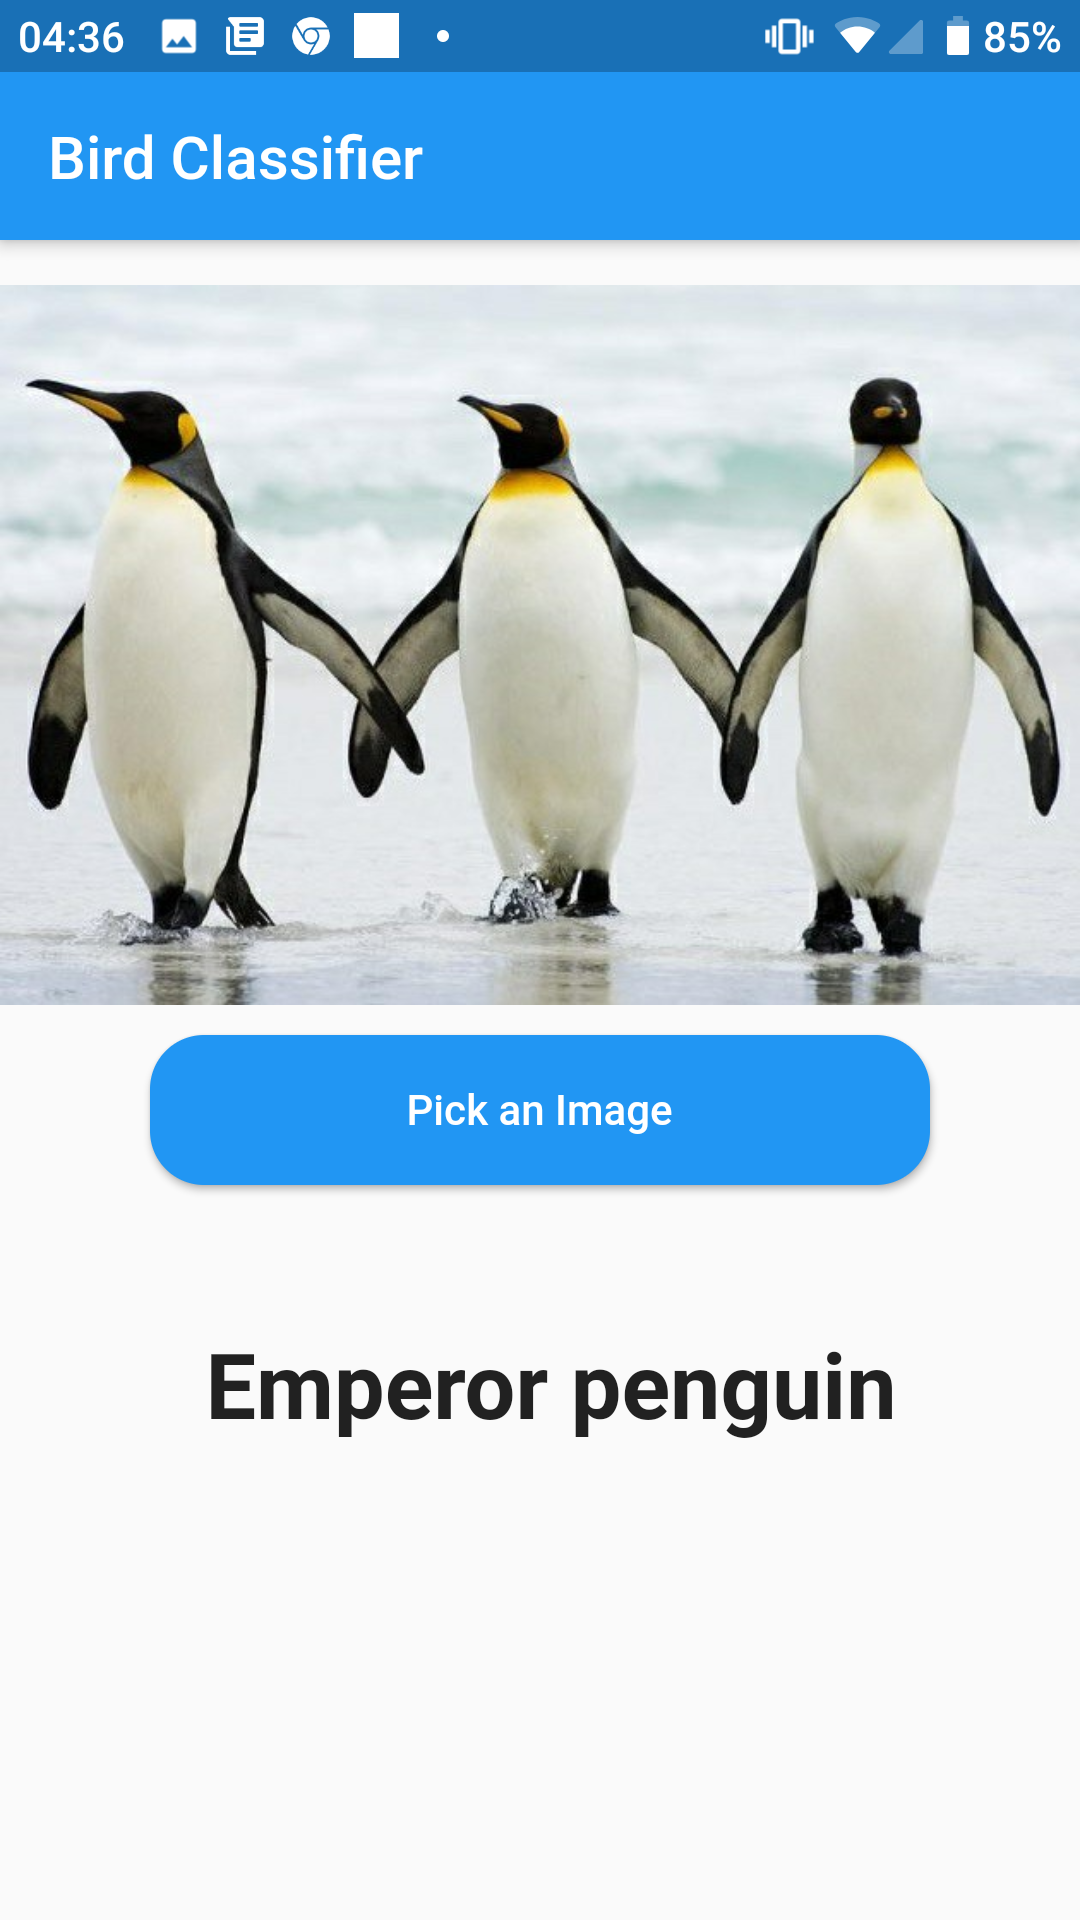
\includegraphics[width = 1.5in]{images/penguin.png}} 
\subfloat[fig 2]{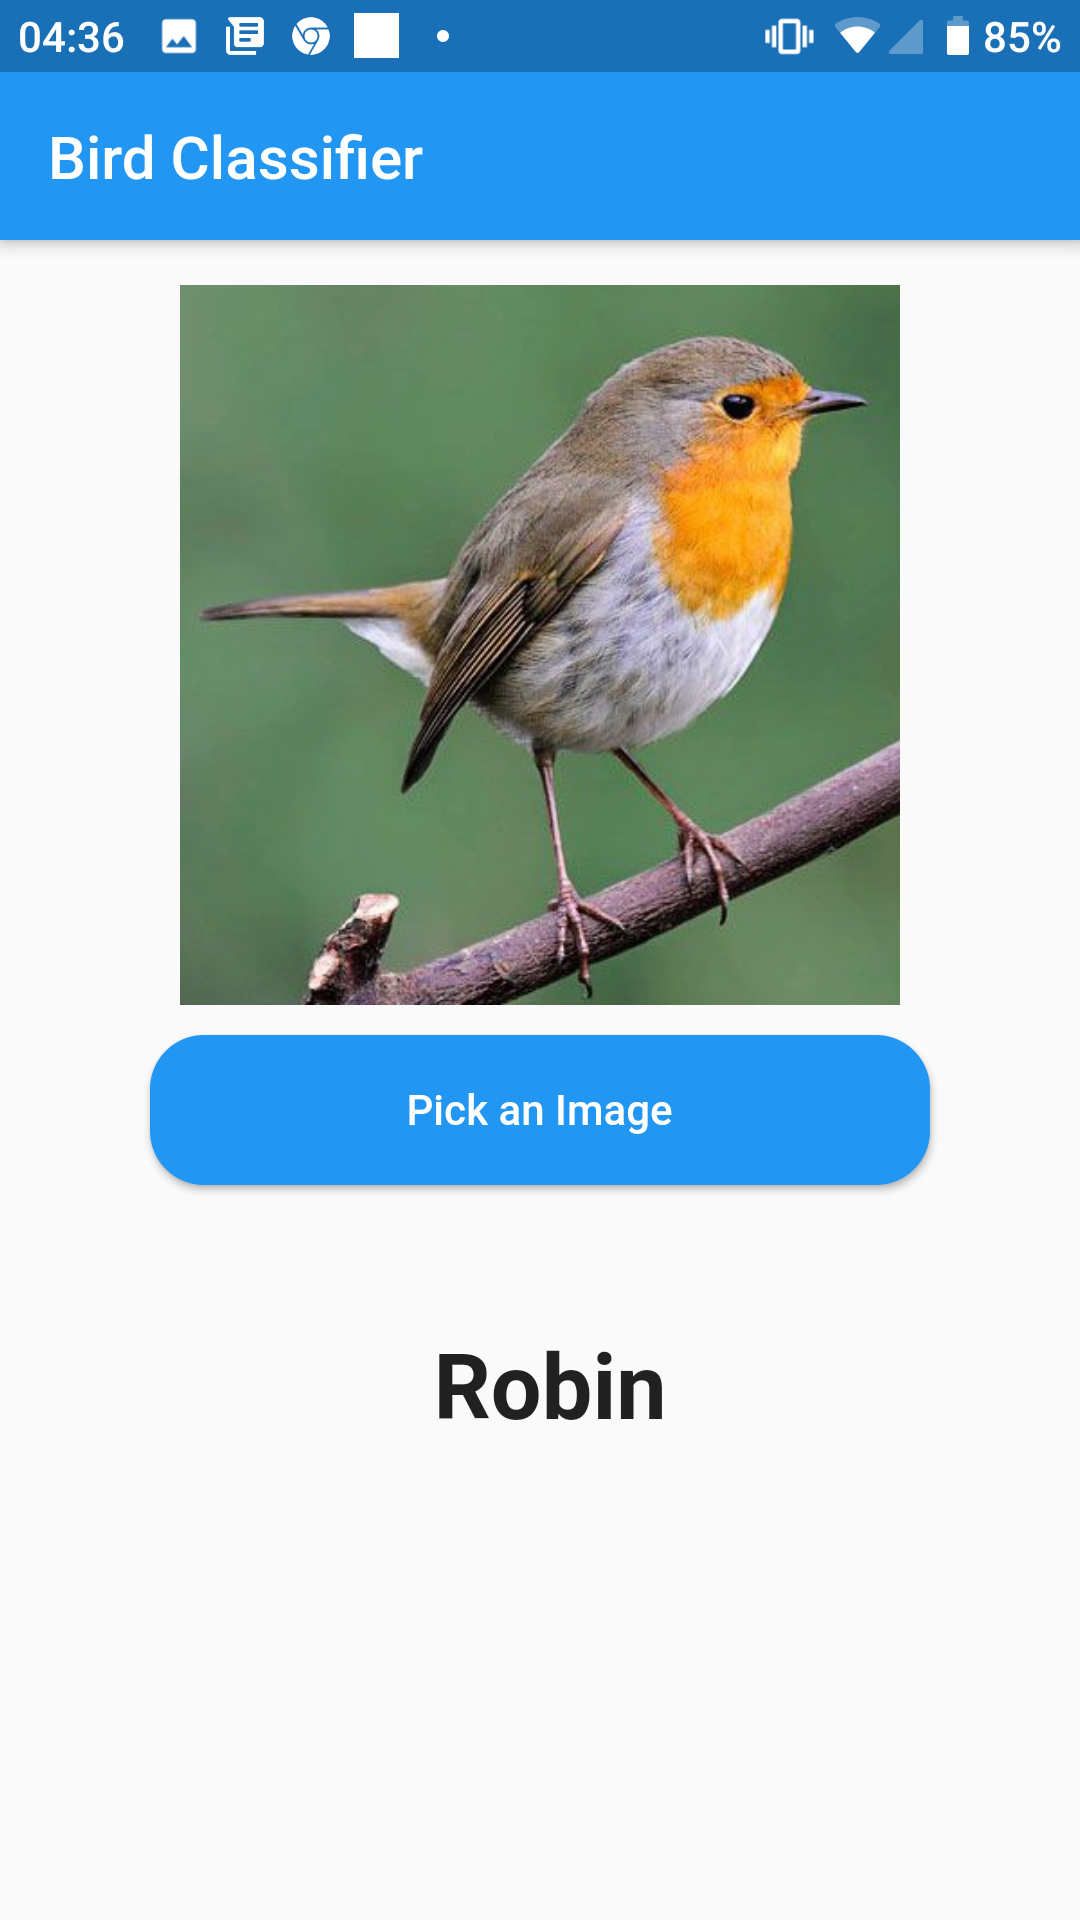
\includegraphics[width = 1.5in]{images/robin.png}}\\
\qquad
\subfloat[fig 3]{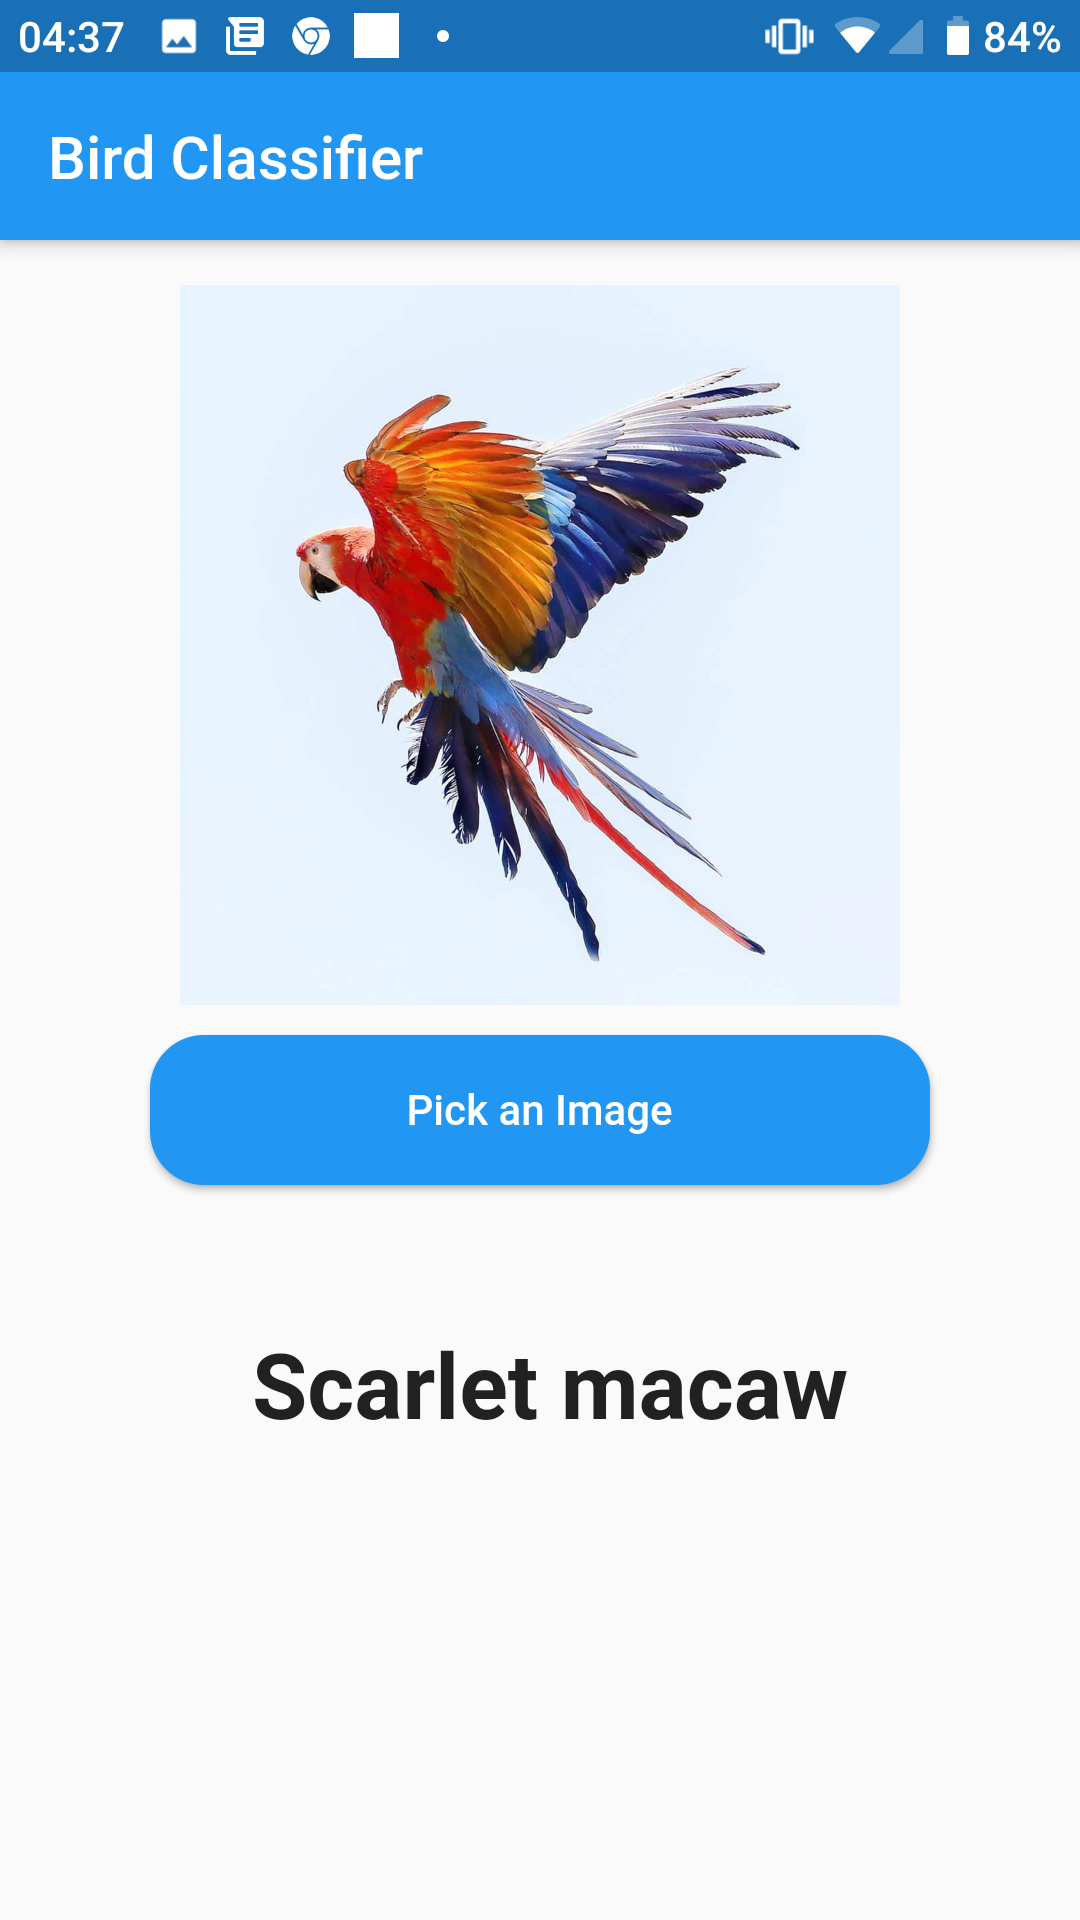
\includegraphics[width = 1.5in]{images/ara.png}}
\subfloat[fig 4]{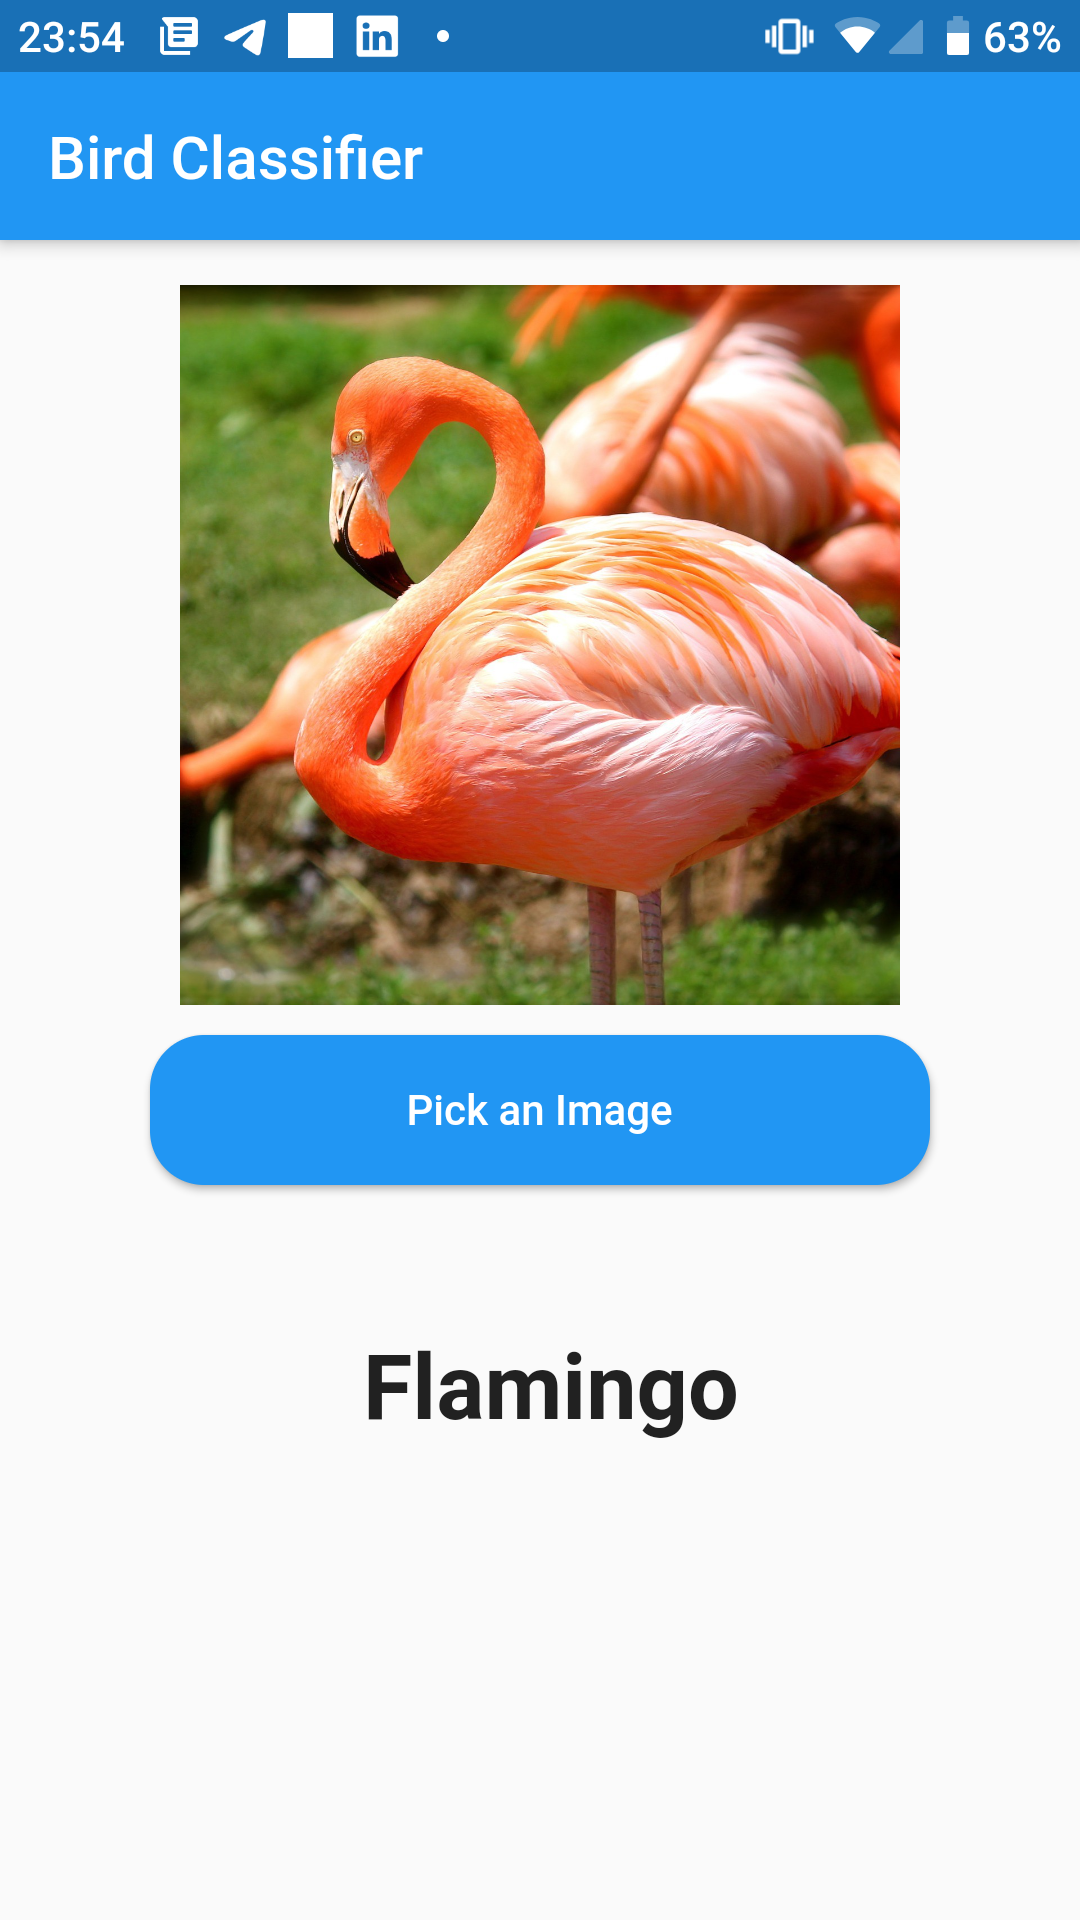
\includegraphics[width = 1.5in]{images/flamingo.png}} 
\caption{The main page of the Application}
\label{some example}
\end{figure}

This is the home of the application, we have a button that allows you to select an image from the gallery or from the camera, then the image can be cropped in order to eliminate the disturbing elements (I remember that the training dataset was composed by cropped images) and finally we will have our prediction. Now let's see the other screens.
\begin{figure}[h!]
\centering
\subfloat[]{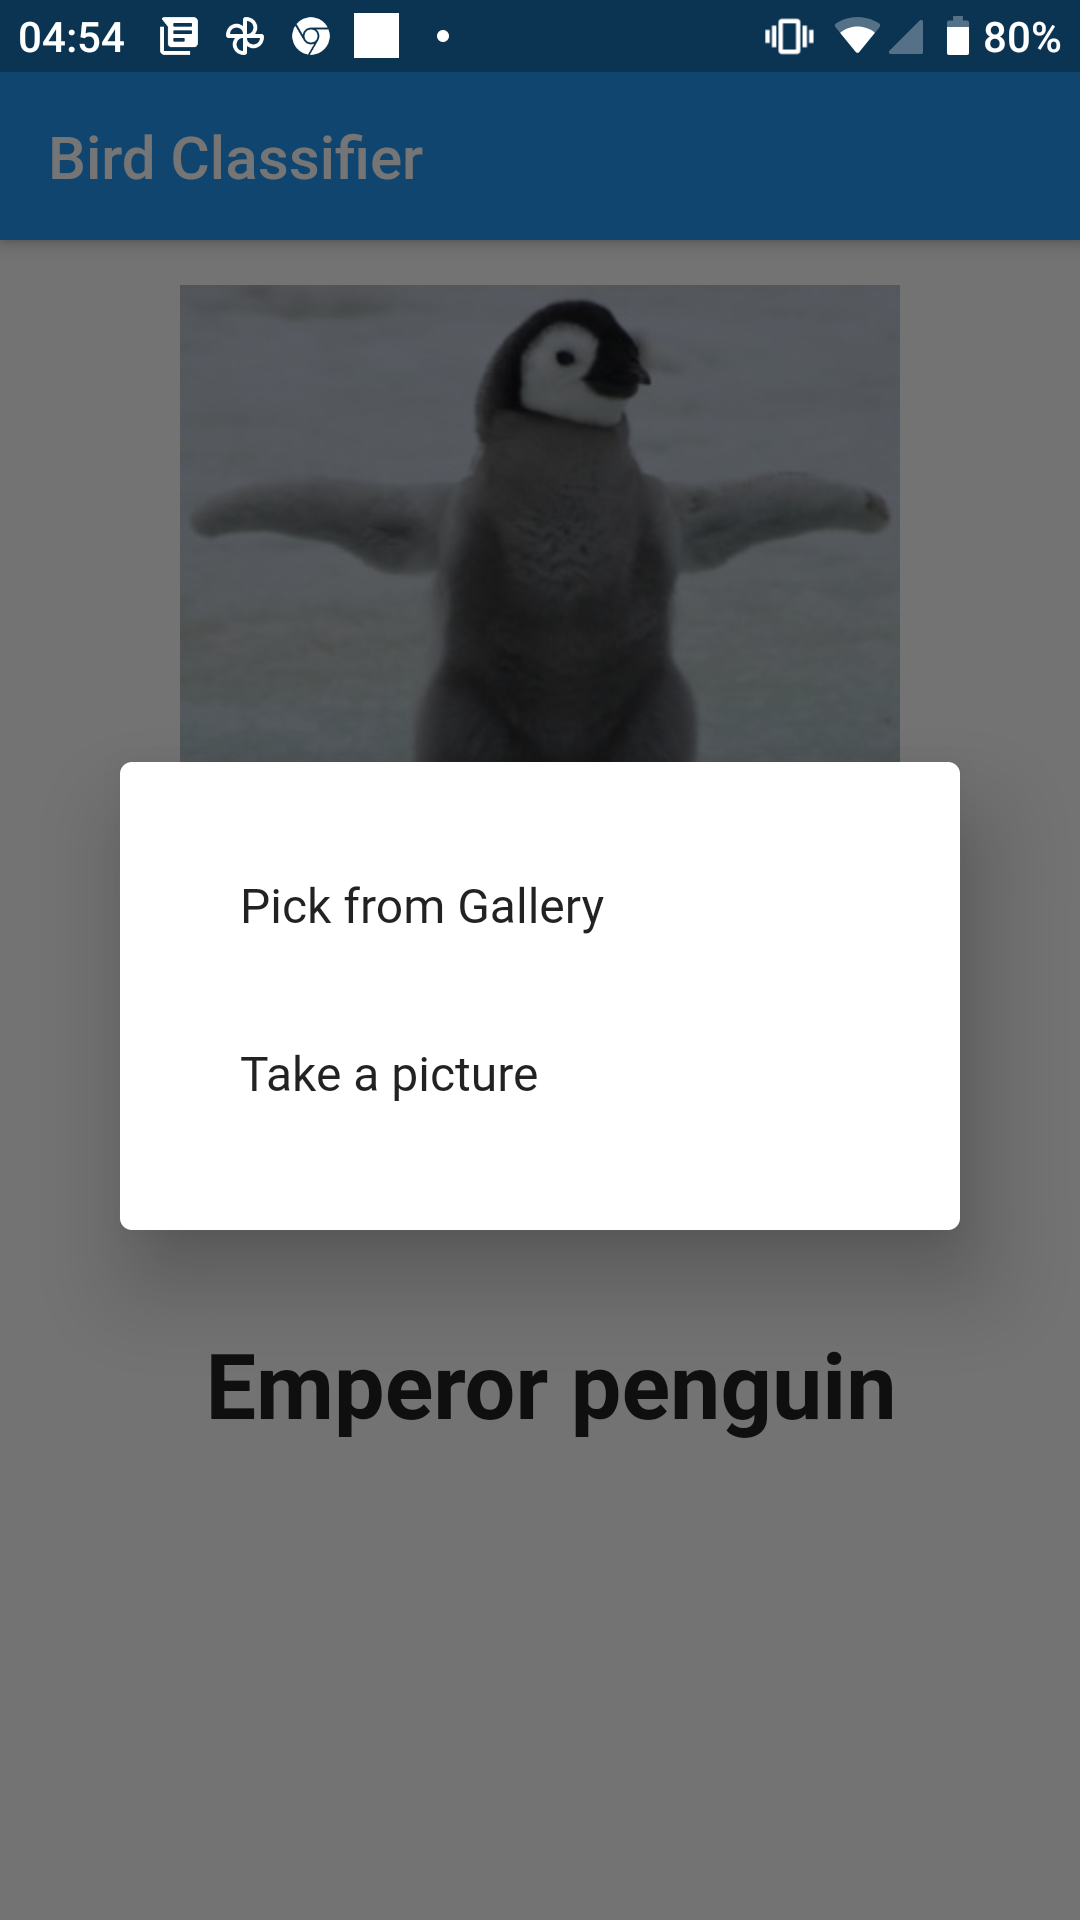
\includegraphics[width = 1.5in]{images/select.png}\label{Select an image}}%
\subfloat[]{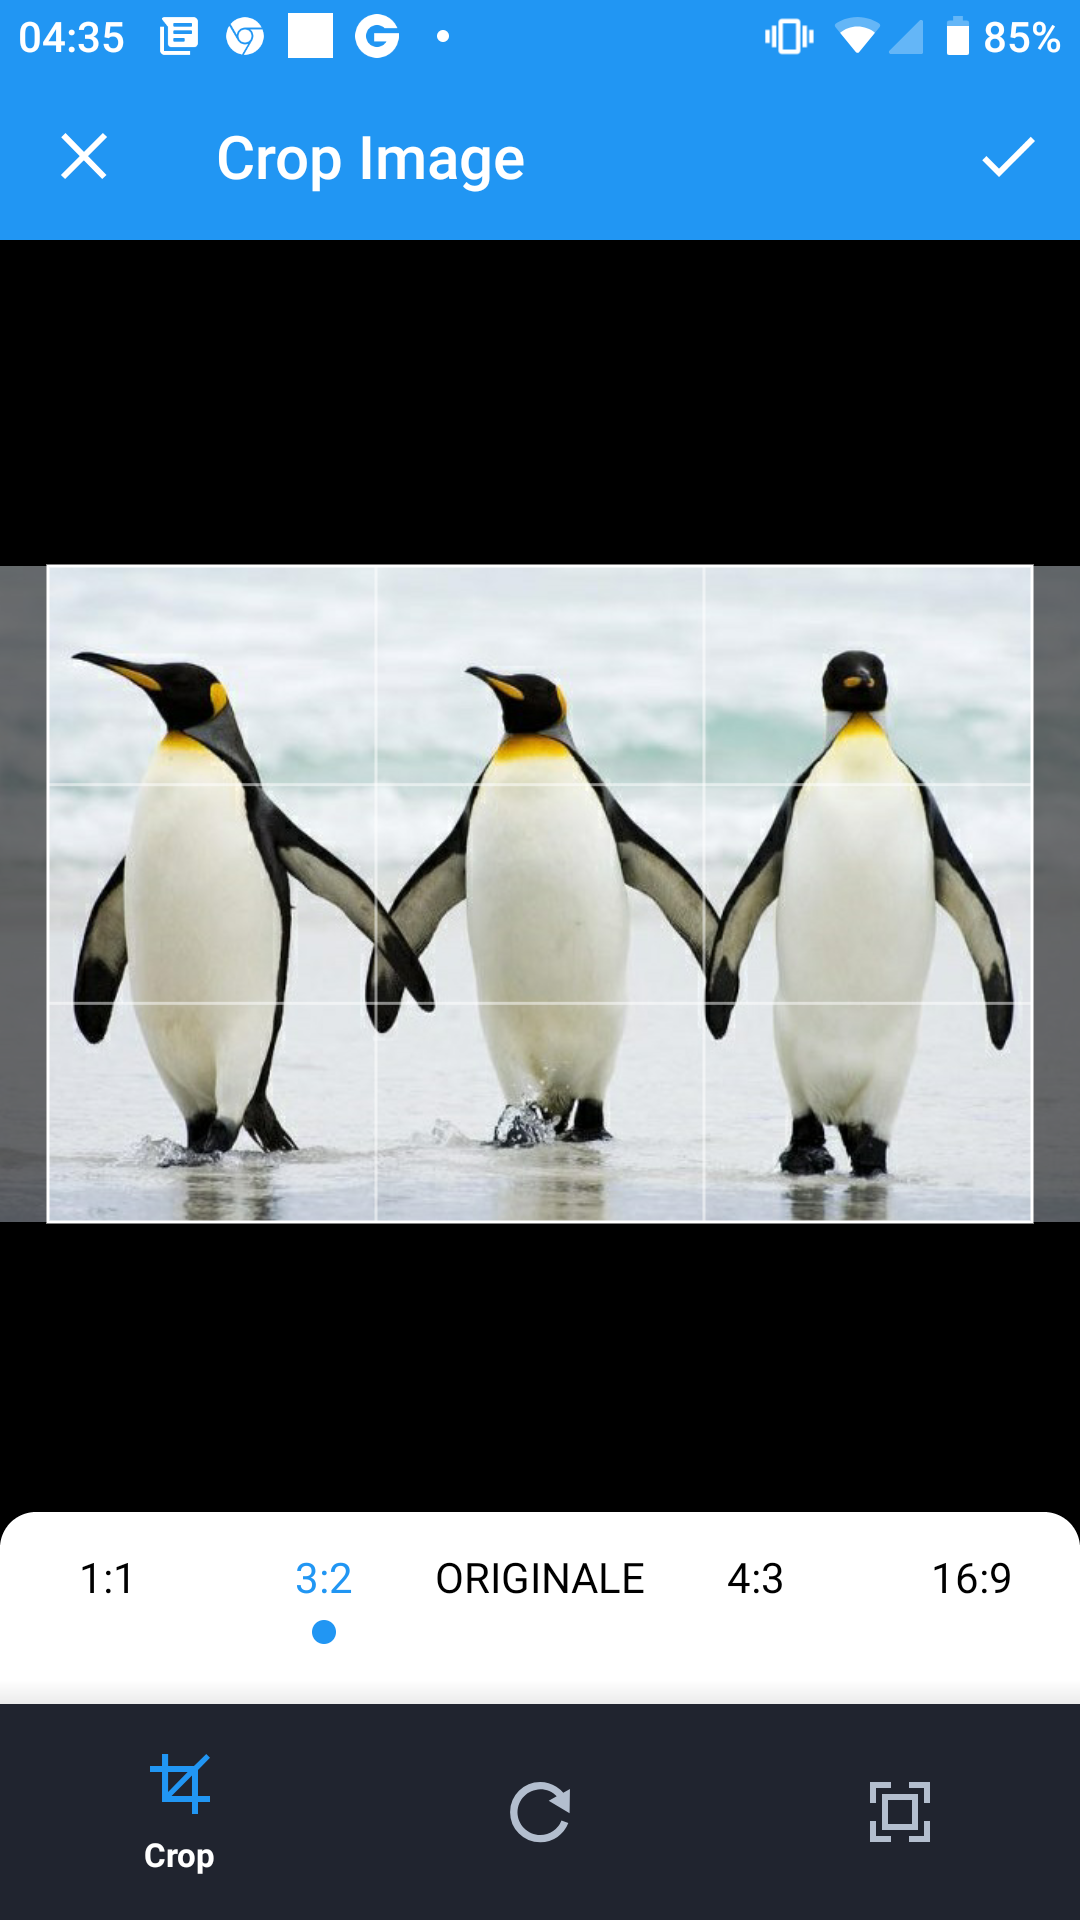
\includegraphics[width = 1.5in]{images/crop.png}\label{Crop the selected image}}\\

\caption{Crop and select functions}
\label{some example}
\end{figure}